%%%%%%%%%%%%%%%%%%%%%%%%%%%%%%%%%%%%
%%                                %%
%%       Structured Dagger        %%
%%                                %%
%%%%%%%%%%%%%%%%%%%%%%%%%%%%%%%%%%%%

\begin{frame}[fragile]
  \frametitle{Chares are reactive}
  \begin{itemize}
    \item The way we described Charm++ so far, a chare is a reactive entity:
      \begin{itemize}
      \item If it gets this method invocation, it does this action,
      \item If it gets that method invocation then it does that action
      \item But what does it do?
      \item In typical programs, chares have a \emph{life-cycle}
      \end{itemize}
    \item How to express the life-cycle of a chare in code?
      \begin{itemize}
      \item Only when it exists
        \begin{itemize}
        \item i.e. some chars may be truly reactive, and the programmer does
          not know the life cycle
        \end{itemize}
      \item But when it exists, its form is:
        \begin{itemize}
        \item Computations depend on remote method invocations, and completion
          of other local computations
        \item A DAG (Directed Acyclic Graph)!
        \end{itemize}
      \end{itemize}
  \end{itemize}
\end{frame}

\begin{frame}
  \frametitle{Consider Fibonacci Chare}
  \begin{itemize}
  \item The Fibonacci chare gets created
  \item If its not a leaf,
    \begin{itemize}
    \item It fires two chares
    \item When both children return results (by calling \code{response}):
      \begin{itemize}
      \item It can compute my result and send it up, or print it
      \end{itemize}
    \item But in our, this logic is hidden in the flags and counters $\ldots$
      \begin{itemize}
      \item This is simple for this simple example, but $\ldots$
      \end{itemize}
    \item Lets look at how this would look with a little notational support
    \end{itemize}
  \end{itemize}
\end{frame}

% \begin{frame}[fragile]
%   \frametitle{What is Structured Dagger?}
%   \begin{itemize}
%     \item Describe in a sequence the flow of control for a parallel object
%     \item Explicitly order and count message delivery and the blocks of code to
%       executed under the proper conditions
%   \end{itemize}
% \end{frame} 

%if -> while -> for
\begin{frame}[fragile]
  \frametitle{Structured Dagger}
  \framesubtitle{The \code{when} construct}
  \begin{itemize}
    \item The \code{when} construct
      \begin{itemize}
        \item Declare the actions to perform when a message is received
        \item In sequence, it acts like a blocking receive
      \end{itemize}
      \begin{lstlisting}[basicstyle=\normalsize]
entry void someMethod() {
  when entryMethod1(parameters) { /* block2 */ }
  when entryMethod2(parameters) { /* block3 */ }
};
      \end{lstlisting}
    \end{itemize}
\end{frame}

\begin{frame}[fragile]
  \frametitle{Structured Dagger}
  \framesubtitle{The \code{serial} construct}
  \begin{itemize}
    \item The \code{serial} construct
      \begin{itemize}
        \item A sequential block of C++ code in the .ci file
        \item The keyword \code{serial} means that the code block will be
          executed without interruption/preemption, like an entry method
        \item Syntax: \code{serial <optionalString> \{ /* C++ code */ \}}
        \item The \code{<optionalString>} is used for identifying the
          \code{serial} for performance analysis
        \item Serial blocks can access all members of the class they belong to
      \end{itemize}
    \item Examples (.ci file):
  \begin{columns}
    \begin{column}{0.5\textwidth}
      \begin{lstlisting}[basicstyle=\tiny]
entry void method1(parameters) {
  serial {
    thisProxy.invokeMethod(10);
    callSomeFunction();
  }
};
      \end{lstlisting}
    \end{column}
    \begin{column}{0.5\textwidth}
      \begin{lstlisting}[basicstyle=\tiny]
entry void method2(parameters) {
  serial "setValue" {
    value = 10;
  }
};
      \end{lstlisting}
    \end{column}
  \end{columns}
  \end{itemize}
\end{frame}


\begin{frame}[fragile]
  \frametitle{Structured Dagger}
  \framesubtitle{The \code{when} construct}
      \begin{lstlisting}[basicstyle=\tiny]
entry void someMethod() {
  serial { /* block1 */ }
  when entryMethod1(parameters) serial { /* block2 */ }
  when entryMethod2(parameters) serial { /* block3 */ }
};
      \end{lstlisting}
  \begin{itemize}
    \item Sequence
      \pause
      \begin{itemize}
        \item Sequentially execute \code{/* block1 */}
          \pause
        \item Wait for \code{entryMethod1} to arrive, if it has not, return control
          back to the Charm++ scheduler, otherwise, execute \code{/* block2 */}
          \pause
        \item Wait for \code{entryMethod2} to arrive, if it has not, return control
          back to the Charm++ scheduler, otherwise, execute \code{/* block3 */}
      \end{itemize}
    \end{itemize}
\end{frame}

\begin{frame}[fragile]
  \frametitle{Structured Dagger}
  \framesubtitle{The \code{when} construct}
  \begin{itemize}
  \item Execute \code{/* further sdag */} when \code{myMethod} arrives
  \begin{lstlisting}[basicstyle=\scriptsize]
when myMethod(int param1, int param2)
  /* further code */
  \end{lstlisting}

  \item Execute \code{/* further sdag */} when \code{myMethod1} and \code{myMethod2} arrive
  \begin{lstlisting}[basicstyle=\scriptsize]
when myMethod1(int param1, int param2),
      myMethod2(bool param3)
  /* further code */
  \end{lstlisting}

\item Which is almost the same as this:
  \begin{lstlisting}[basicstyle=\scriptsize]
when myMethod1(int param1, int param2) {
  when myMethod2(bool param3) { }
}
    /* further code */
  \end{lstlisting}

  \end{itemize}
\end{frame}

\begin{frame}
  \frametitle{Structured Dagger}
  \framesubtitle{Boilerplate}
  \begin{itemize}
    \item Structured Dagger can be used in any entry method (except for a constructor)
      \begin{itemize}
      \item Can be used in a \code{mainchare}, \code{chare}, or \code{array}
      \end{itemize}
    \item For any class that has Structured Dagger in it you must insert two
      calls:
       \begin{itemize}
         \item The Structured Dagger macro: \code{[ClassName]\_SDAG\_CODE}
%         \item Call the \code{\_\_sdag\_init()} initializer in the constructor
         \item For later: call the \code{\_\_sdag\_pup()} in the \code{pup} method
       \end{itemize}
  \end{itemize}
\end{frame}

\begin{frame}[fragile]
  \frametitle{Structured Dagger}
  \framesubtitle{Boilerplate}
  The .ci file:
  \begin{lstlisting}
    [mainchare,chare,array] MyFoo {
      ...
      entry void method(parameters) {
        // ... structured dagger code here ...
      };
      ...
    }
  \end{lstlisting}

  The .cpp file:
  \begin{lstlisting}
    class MyFoo : public CBase_MyFoo {
      MyFoo_SDAG_CODE /* insert SDAG macro */
    public:
      MyFoo() { }
    };
  \end{lstlisting}
\end{frame}

\begin{frame}[fragile]
  \frametitle{Fibonacci with Structured Dagger}
  \lstinputlisting[basicstyle=\scriptsize]{code/fibSDAG.ci}
\end{frame}

\begin{frame}[fragile]
  \frametitle{Fibonacci with Structured Dagger}
  \lstinputlisting[basicstyle=\tiny]{code/fibSDAG.cc}
\end{frame}

\begin{frame}[fragile]
  \frametitle{Structured Dagger}
  \framesubtitle{The \code{when} construct}
\begin{itemize}
  \item What is the sequence?
  \begin{lstlisting}[basicstyle=\scriptsize]
when myMethod1(int param1, int param2) {
  when myMethod2(bool param3),
        myMethod3(int size, int arr[size]) /* sdag block1 */
  when myMethod4(bool param4) /* sdag block2 */
}
  \end{lstlisting}
  \pause
  \item Sequence:
    \begin{itemize}
      \item Wait for \code{myMethod1}, upon arrival execute body of \code{myMethod1}
        \pause
      \item Wait for \code{myMethod2} and \code{myMethod3}, upon arrival of
        both, execute \code{/* sdag block1 */}
        \pause
      \item Wait for \code{myMethod4}, upon arrival execute \code{/* sdag block2 */}
    \end{itemize}
  \item Question: if \code{myMethod4} arrives first what will happen?
\end{itemize}

\end{frame}

% \begin{frame}[fragile]
%   \frametitle{Structured Dagger Constructs: Reference Numbers}
%   \begin{itemize}
%     \item Entry methods can be \emph{tagged} with a \emph{reference number}
%     \item A reference number is a special field in the envelope of the message
%       that is sent
%     \item By default, the reference number is a \code{short}
%     \item This can be changed when compiling charm:
%       \begin{itemize}
%       \item Add this to the build flags:
%         \code{--with-refnum-type=int}
%       \item For example, compiling on BG/P with the IBM XLC compiler:

%       \end{itemize}
%   \end{itemize}
% \code{./build charm++ bluegenep xlc --with-refnum-type=int -g -O0}

% \end{frame}

\begin{frame}[fragile]
  \frametitle{Structured Dagger Constructs}
  \framesubtitle{The \code{when} construct}
  \begin{itemize}
    \item The \code{when} clause can wait on a certain reference number
    \item If a reference number is specified for a \code{when}, the first
      parameter for the \code{when} must be the reference number
    \item Semantic: the \code{when} will ``block'' until a message arrives with
      that reference number
  \end{itemize}
  \begin{lstlisting}
    when method1[100](int ref, bool param1)
      /* sdag block */

    serial {
      proxy.method1(200, false); /* will not be delivered to the when */
      proxy.method1(100, true);  /* will be delivered to the when */
    }
  \end{lstlisting}
\end{frame}

\begin{frame}[fragile]
  \frametitle{Structured Dagger}
  \framesubtitle{The \code{if-then-else} construct}
  \begin{itemize}
  \item The \code{if-then-else} construct:
    \begin{itemize}
    \item Same as the typical C if-then-else semantics and syntax
    \end{itemize}
  \end{itemize}
  \begin{lstlisting}
  if (thisIndex.x == 10) {
    when method1[block](int ref, bool someVal) /* code block1 */
  } else {
    when method2(int payload) serial {
      //... some C++ code
    }
  }
  \end{lstlisting}
\end{frame}

\begin{frame}[fragile]
  \frametitle{Structured Dagger}
  \framesubtitle{The \code{for} construct}
  \begin{itemize}
  \item The \code{for} construct:
    \begin{itemize}
    \item Defines a sequenced \code{for} loop (like a sequential C for loop)
    \item Once the body for the $i$th iteration completes, the $i+1$ iteration
      is started
    \end{itemize}
  \end{itemize}
  \begin{lstlisting}
    for (iter = 0; iter < maxIter; ++iter) {
      when recvLeft[iter](int num, int len, double data[len])
        serial { computeKernel(LEFT, data); }
      when recvRight[iter](int num, int len, double data[len])
        serial { computeKernel(RIGHT, data); }
    }
  \end{lstlisting}
  \begin{itemize}
  \item \code{iter} must be defined in the class as a member
  \end{itemize}
  \begin{lstlisting}
    class Foo : public CBase_Foo {
      public: int iter;
    };
  \end{lstlisting}
\end{frame}

\begin{frame}[fragile]
  \frametitle{Structured Dagger}
  \framesubtitle{The \code{while} construct}
  \begin{itemize}
  \item The \code{while} construct:
    \begin{itemize}
    \item Defines a sequenced \code{while} loop (like a sequential C while loop)
    \end{itemize}
  \end{itemize}
  \begin{lstlisting}
    while (i < numNeighbors) {
      when recvData(int len, double data[len]) {
        serial {
          /* do something */
        }
        when method1() /* block1 */
        when method2() /* block2 */
      }
      serial { i++; }
    }
  \end{lstlisting}
\end{frame}

% \begin{frame}[fragile]
%   \frametitle{Structured Dagger Constructs: \code{when}}
%   \begin{itemize}
%   \item Another example:
%   \end{itemize}
%   .ci file:
%   \begin{lstlisting}
%     chare MyChare {
%       entry MyChare();
%       entry void startWork() {
%         serial { myRef = 100; }
%         when method1[myRef1](int ref, bool param1) /*  block1 */
%         when method2[myRef2](int ref, bool param1) /* block2 */
%       };
%     }
%   \end{lstlisting}
%   .cpp file:
%   \begin{lstlisting}
%     class MyChare : public CBase_MyChare {
%        int myRef1, myRef2;
%        MyChare() : myRef2(200) { }
%     };
%   \end{lstlisting}
% \end{frame}

\begin{frame}[fragile]
  \frametitle{Structured Dagger}
  \framesubtitle{The \code{overlap} construct}
  \begin{itemize}
  \item The \code{overlap} construct:
    \begin{itemize}
    \item By default, Structured Dagger defines a sequence that is followed sequentially
    \item \code{overlap} allows multiple independent clauses to execute in any order
    \item Any constructs in the body of an \code{overlap} can happen in any
      order
    \item An \code{overlap} finishes in sequence when all the statements in it
      are executed
    \item Syntax: \code{overlap \{ /* sdag constructs */ \}}
    \end{itemize}
  \end{itemize}
  What are the possible execution sequences?
  \begin{lstlisting}
    serial { /* block1 */ }
    overlap {
      serial { /* block2 */ }
      when entryMethod1[100](int ref_num, bool param1) /* block3 */
      when entryMethod2(char myChar) /* block4 */
    }
    serial { /* block5 */ }
  \end{lstlisting}
\end{frame}

\begin{frame}
  \frametitle{Illustration of a long ``overlap''}
  \begin{columns}
    \begin{column}{0.6\textwidth}
      \begin{itemize}
      \item Overlap can be used to get back some of the asynchrony within a chare
        \begin{itemize}
        \item But it is constrained
        \item Makes for more disciplined programming, 
          \begin{itemize}
          \item with fewer race conditions
          \end{itemize}
        \end{itemize}
      \end{itemize}
    \end{column}
    \begin{column}{0.4\textwidth}
      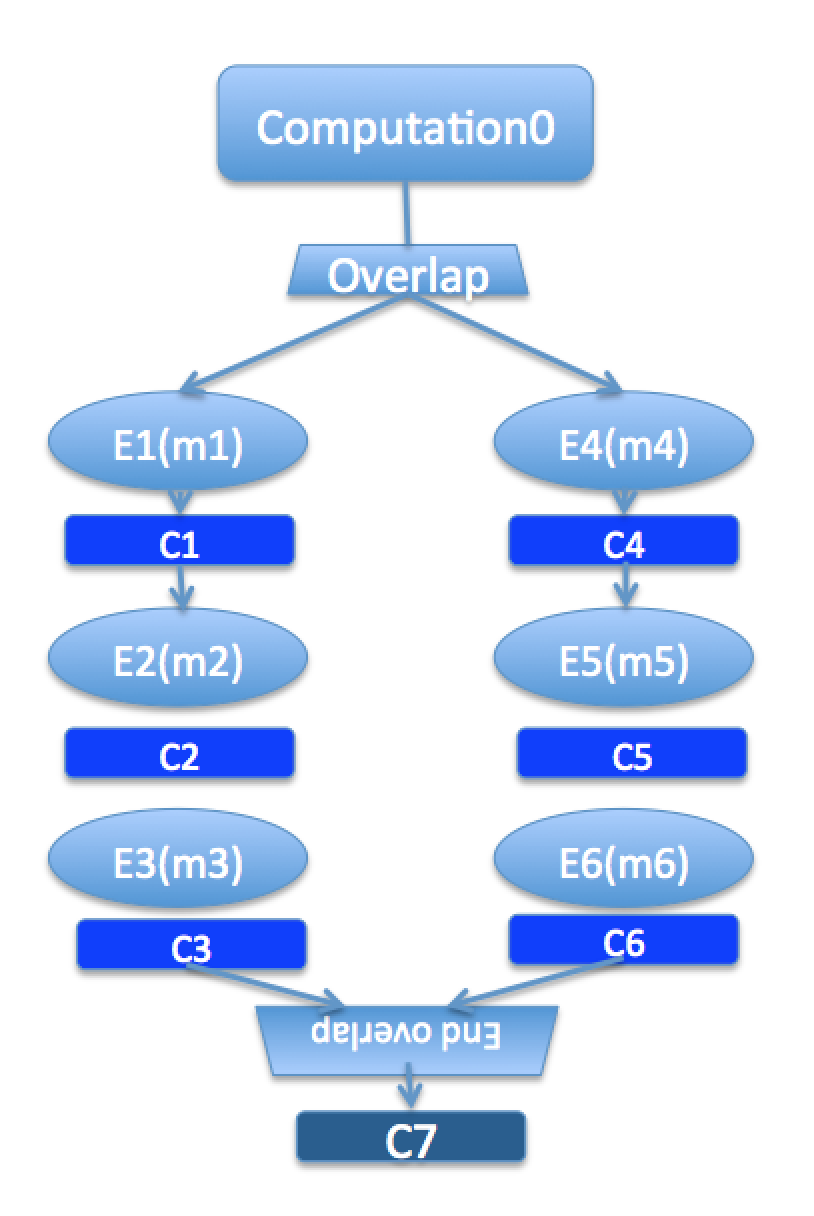
\includegraphics[width=0.8\textwidth]{figures/overlapFlow.png}
    \end{column}
  \end{columns}
\end{frame}

\begin{frame}[fragile]
  \frametitle{Structured Dagger}
  \framesubtitle{The \code{forall} construct}
  \begin{itemize}
  \item The \code{forall} construct:
    \begin{itemize}
    \item Has ``do-all'' semantics: iterations may execute an any order
    \item Syntax: \code{forall [<ident>] (<min> : <max>, <stride>) <body>}
    \item The range from \code{<min>} to \code{<max>} is inclusive
    \end{itemize}
  \end{itemize}
  \begin{lstlisting}
    forall [block] (0 : numBlocks - 1, 1) {
      when method1[block](int ref, bool someVal) /* code block1 */
    }
  \end{lstlisting}
  \begin{itemize}
    \item Assume \code{block} is declared in the class as \code{public: int block;}
  \end{itemize}
\end{frame}

% \begin{frame}[fragile]
%   \frametitle{Determinant MP0 Solution: .ci file}
%   \lstinputlisting[basicstyle=\footnotesize]{code/det.ci}
% \end{frame}

% \begin{frame}[fragile]
%   \frametitle{Determinant MP0 Solution: .cpp file (part 1)}
%   \lstinputlisting[basicstyle=\tiny]{code/detp1.C}
% \end{frame}

% \begin{frame}[fragile]
%   \frametitle{Determinant MP0 Solution: .cpp file (part 2)}
%   \lstinputlisting[basicstyle=\tiny]{code/detp2.C}
% \end{frame}

% \begin{frame}[fragile]
%   \frametitle{Determinant MP0 Structered Dagger: .ci file}
%   \lstinputlisting[basicstyle=\scriptsize]{code/detSDAG.ci}
% \end{frame}

% \begin{frame}[fragile]
%   \frametitle{Determinant MP0 Structered Dagger: .cpp file}
%   \lstinputlisting[basicstyle=\tiny]{code/detSDAG.C}
% \end{frame}

\begin{frame}[fragile]
  \frametitle{5-point Stencil}
   \begin{center} 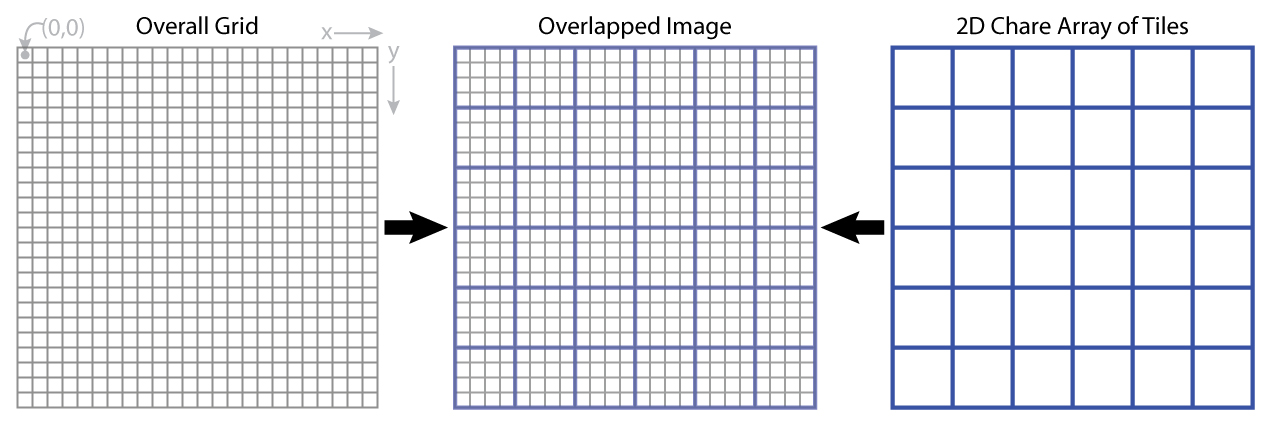
\includegraphics[width=0.85\textwidth]{figures/2DJacobi_Decomposition.jpg} \end{center}
\end{frame}

\begin{frame}[fragile]
  \frametitle{5-point Stencil}
   \begin{center} 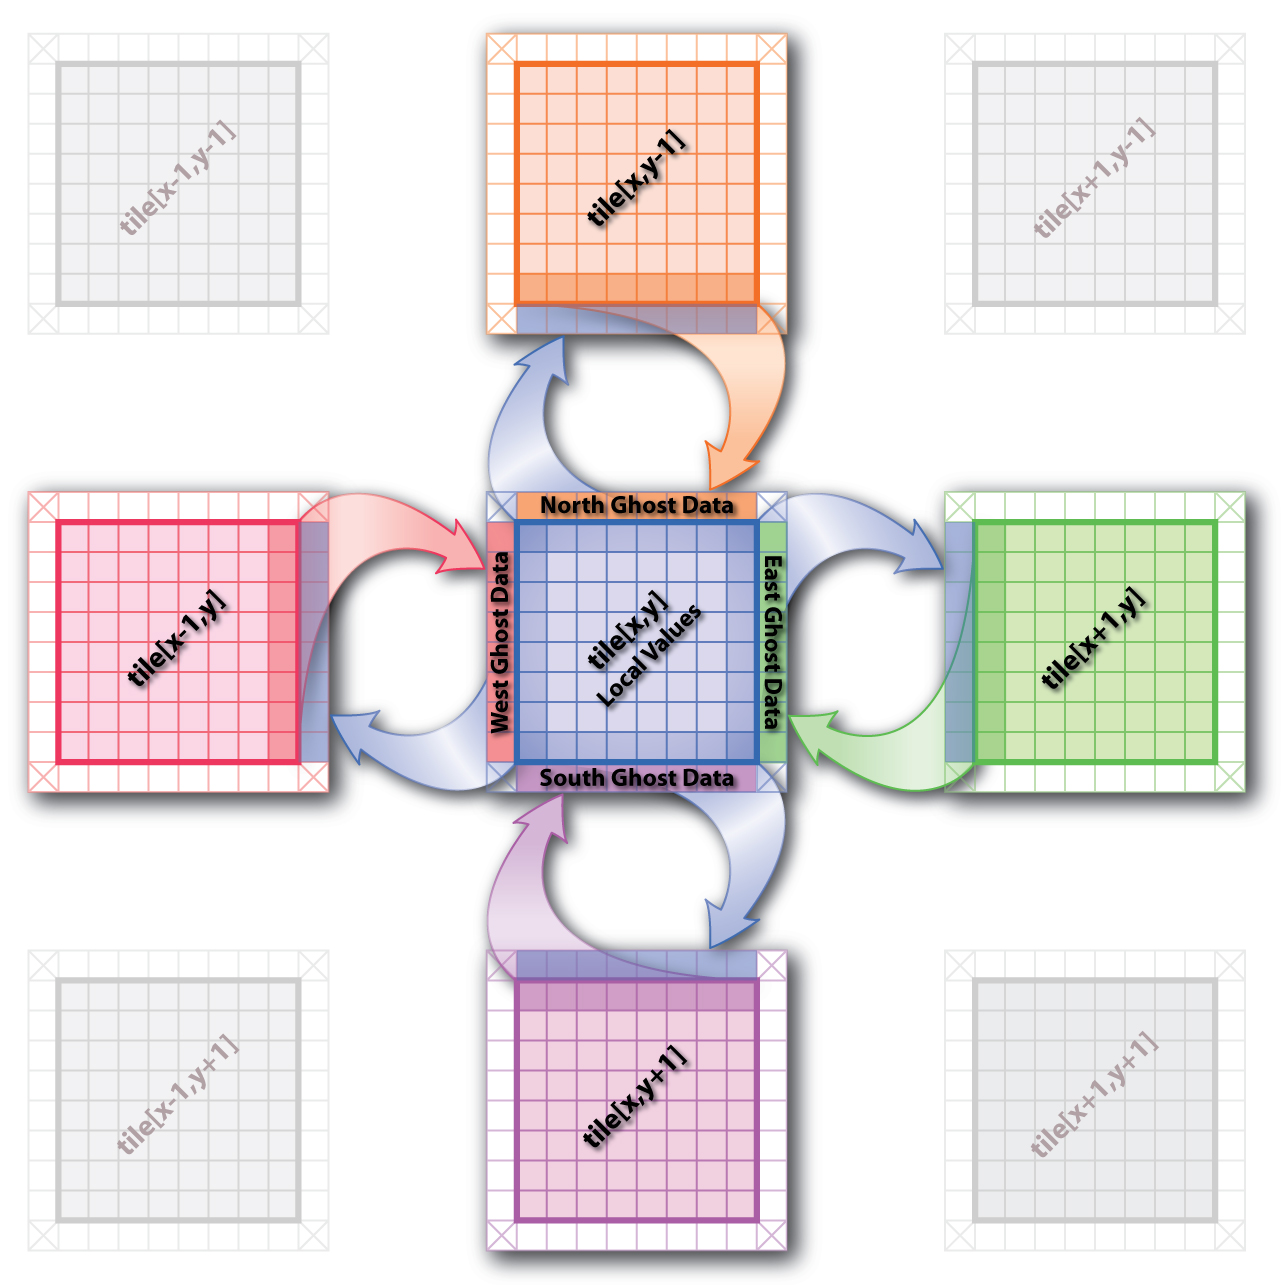
\includegraphics[width=0.6\textwidth]{figures/2DJacobi_NeighborComm.jpg} \end{center}
\end{frame}

\begin{frame}[fragile]
  \frametitle{5-point Stencil}
   \begin{center} 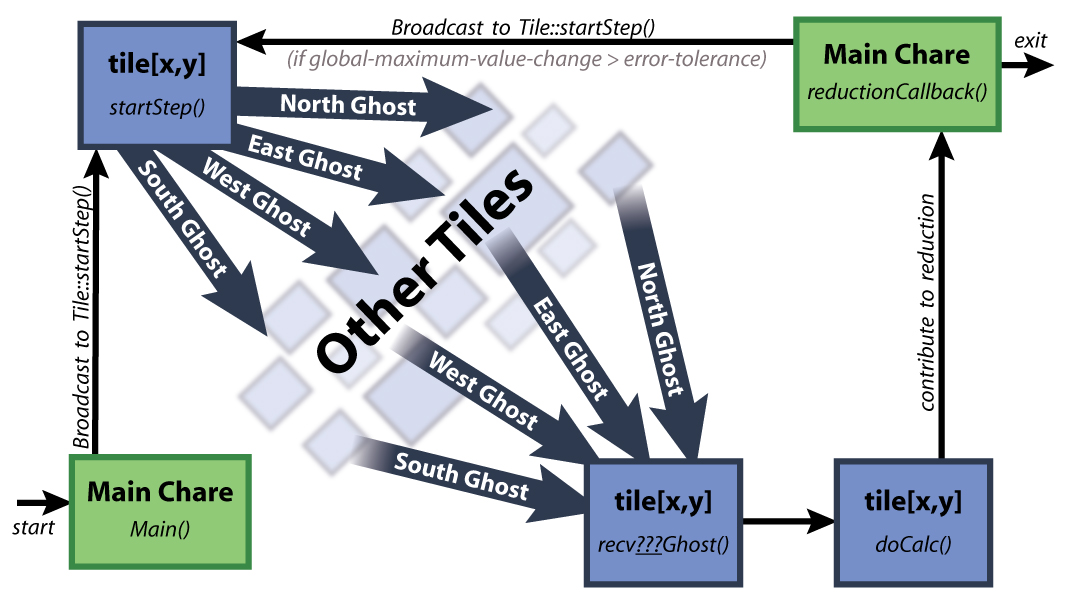
\includegraphics[width=0.8\textwidth]{figures/2DJacobi_LogicFlow.jpg} \end{center}
\end{frame}

\begin{frame}[fragile]
  \frametitle{Jacobi: .ci file}
  \lstinputlisting[basicstyle=\footnotesize]{code/jacobi3dELL.ci}
\end{frame}

\begin{frame}[fragile]
  \frametitle{Jacobi: .ci file}
  \lstinputlisting[basicstyle=\tiny,linerange={22-49}]{code/jacobi3dSYNC.ci}
\end{frame}

\begin{frame}[fragile]
  \frametitle{Jacobi: .ci file (with \textbf{asynchronous} reductions)}
  \lstinputlisting[basicstyle=\tiny,linerange={22-50}]{code/jacobi3d.ci}
\end{frame}

% \begin{frame}[fragile]
%   \frametitle{Jacobi: .cpp file}
%   \lstinputlisting[basicstyle=\tiny,linerange={40-46,89-103}]{code/jacobi3d.C}
% \end{frame}

% \begin{frame}[fragile]
%   \frametitle{Jacobi: .cpp file}
%   \lstinputlisting[basicstyle=\tiny,linerange={109-139}]{code/jacobi3d.C}
% \end{frame}

% \begin{frame}[fragile]
%   \frametitle{Jacobi: .cpp file}
%   \lstinputlisting[basicstyle=\tiny,linerange={109-138}]{code/jacobi3d.C}
% \end{frame}

% \begin{frame}[fragile]
%   \frametitle{Jacobi: .cpp file}
%   \lstinputlisting[basicstyle=\tiny,linerange={164-190}]{code/jacobi3d.C}
% \end{frame}

% \begin{frame}[fragile]
%   \frametitle{Jacobi: .cpp file}
%   \lstinputlisting[basicstyle=\tiny,linerange={201-230}]{code/jacobi3d.C}
% \end{frame}